\documentclass[11pt]{report}
\usepackage{geometry}                % See geometry.pdf to learn the layout options. There are lots.
\geometry{a4paper}                   % ... or a4paper or a5paper or ...
%\geometry{landscape}                % Activate for for rotated page geometry
%\usepackage[parfill]{parskip}    % Activate to begin paragraphs with an empty line rather than an indent
\usepackage{graphicx}
\usepackage{amssymb}
\usepackage{epstopdf}
\DeclareGraphicsRule{.tif}{png}{.png}{`convert #1 `dirname #1`/`basename #1 .tif`.png}

\usepackage[colorlinks]{hyperref}
\usepackage{underscore}
\usepackage{textcomp}
\usepackage{xcolor}
\usepackage{parskip}
\usepackage{framed}
\usepackage{listings}
\usepackage[nosolutionfiles]{answers}
\usepackage{tikz}
\usetikzlibrary{arrows,automata,shapes,snakes,patterns,decorations}
\usetikzlibrary{shapes.geometric,shapes.misc}
\usetikzlibrary{shadows}
\usetikzlibrary{calc}
\usetikzlibrary{positioning}
\usepackage{adjustbox}

\lstset{
  language=C,
  basicstyle=\ttfamily\footnotesize,
  commentstyle=\itshape\color{cyan},
  frame=lines
}


\Newassociation{sol}{Solution}{ans}
\newtheorem{ex}{Question}

\newcommand{\normaltilde}{{\raise.17ex\hbox{$\scriptstyle\mathtt{\sim}$}}}
\newcommand{\unixcl}[1]{\texttt{\fcolorbox{black}{gray!20}{\footnotesize#1}}}
\newcommand{\blanc}{\fcolorbox{white}{white}{~}}
\newcommand{\tabkey}{\mbox{$\rightarrow\hspace{-1.4mm}\vert$}}
\title{Real-time programming labs\\IMTA, option AII, 2018-2019}
\author{Jean-Luc B\'echennec, S\'ebastien Faucou}
%\date{}                                           % Activate to display a given date or no date

\hypersetup{linkcolor=red}

\colorlet{shadecolor}{gray!10}

\begin{document}
\maketitle


\chapter{Installation}

\section{Foreword}

It is assumed that you have a basic knowledge of the Linux environment.
If it is not the case, make sure to have the first configuration steps checked before to proceed with the labs.

\begin{framed}
Do not copy the commands from the PDF file, the characters you get may not have the correct code and the shell will not understand them.
\end{framed}

When typing shell commands, remember that spaces are important because they separate the command and its arguments. In this document, spaces in commands are represented by a white rectangle like in the following command (it is an example, do not type it):

\noindent
\begin{minipage}{.25\textwidth}
\unixcl{cd\blanc{}trampoline}
\end{minipage}
\begin{minipage}{.7\textwidth}
sets the {\tt trampoline} directory as current directory. This assumes the {\tt trampoline} directory is a subdirectory of the current one.
\end{minipage}

A toolchain to build and download programs with Trampoline has been installed on the computers in the \texttt{/usr/local/tp\_treel\_imta}. In this folder, you will find:
\begin{itemize}
    \item a version of Trampoline in the \texttt{trampoline} subfolder; it includes the \texttt{goil} compiler to parse \texttt{OIL} kernel configuration files, the kernel code, and an automated build system.
    \item a cross-compilation chain, namely \texttt{arm-gcc} in the \texttt{gcc-arm-none-eabi-7-2018-q2-update} subfolder.
    \item a tool to download binaries to the target board: \texttt{teensy-loader-cli}.
\end{itemize}

All these tools are open-source (see the licence of each projet for more details) and are available on the following websites:

\begin{itemize}
    \item
        \url{https://github.com/TrampolineRTOS/trampoline}
    \item
        \url{https://launchpad.net/gcc-arm-embedded}
    \item
        \url{https://github.com/PaulStoffregen/teensy_loader_cli}
\end{itemize}


\section{Environment settings}

In order to be able to use the tools, you have to define the configuration of your development environment. First, you have to inform the shell of the location of the tools. This is done by setting the {\tt PATH} environment variable.

Edit the \texttt{.login} file in your home directory add the following lines at the end:


\unixcl{set\blanc{}path=(\$path /usr/local/tp\_treel\_imta/bin /usr/local/tp\_treel\_imta/gcc-arm/bin)}

The \texttt{.login} file is parsed by the shell when it starts. To force your current shell instance to read the file, use the following command:

\unixcl{source\blanc{}\normaltilde/.login}

This will enable the configuration in the terminal where you typed the command.
In order to have the configuration active in all terminals, you have to log out and then log in the system.


Now, test that Goil is working. The command \unixcl{goil\blanc{}--version} should print:

\medskip

\begin{shaded*}
\tiny
\vspace{-1.7mm}
\begin{verbatim}
goil : 2.1.26, build with GALGAS 3.1.3
\end{verbatim}
\end{shaded*}

Test that gcc-arm is also working. The commande \unixcl{arm-none-eabi-gcc\blanc{}--version} should print:

\medskip

\begin{shaded*}
\tiny
\vspace{-1.7mm}
\begin{verbatim}
arm-none-eabi-gcc (GNU Tools for Arm Embedded Processors 7-2018-q2-update) 7.3.1 20180622 (release) [ARM/embedded-7-branch revision 261907]
Copyright (C) 2017 Free Software Foundation, Inc.
This is free software; see the source for copying conditions.  There is NO
warranty; not even for MERCHANTABILITY or FITNESS FOR A PARTICULAR PURPOSE.

\end{verbatim}
\end{shaded*}

Last, test Teensy loader is working. The command \unixcl{teensy-loader-cli} should print:

\medskip

\begin{shaded*}
\tiny
\vspace{-1.7mm}
\begin{verbatim}
Filename must be specified

Usage: teensy_loader_cli --mcu=<MCU> [-w] [-h] [-n] [-b] [-v] <file.hex>
        -w : Wait for device to appear
        -r : Use hard reboot if device not online
        -s : Use soft reboot if device not online (Teensy3.x only)
        -n : No reboot after programming
        -b : Boot only, do not program
        -v : Verbose output

Use `teensy_loader_cli --list-mcus` to list supported MCUs.

For more information, please visit:
http://www.pjrc.com/teensy/loader_cli.html
\end{verbatim}
\end{shaded*}

You are now ready to compile and load your first application on the board. But first, let's take a look at the board.

\chapter{The board}

\section{The Teensy 3.1}
\label{teensy}

The board is built around a Teensy 3.1 breakout board (BB). A breakout board is a minimal board designed to be used with tiny SMD\footnote{Surface Mounted Device} on a breadboard or in a hobbyist design. The Teensy 3.1 BB is built around a Freescale Micro-controller, the MK20DX256VLH7, which has an ARM Cortex-M4 computing core. It is a 32 bits micro-controller running at 96MHz. It embeds 256kB of flash memory to store the program and the constant data and 64kB of SRAM to store the variables. The Teensy is built by PJRC, a small company from the USA. \href{https://www.pjrc.com/teensy/teensy31.html}{The web site is here}. Here is the Teensy 3.1:

\begin{center}
   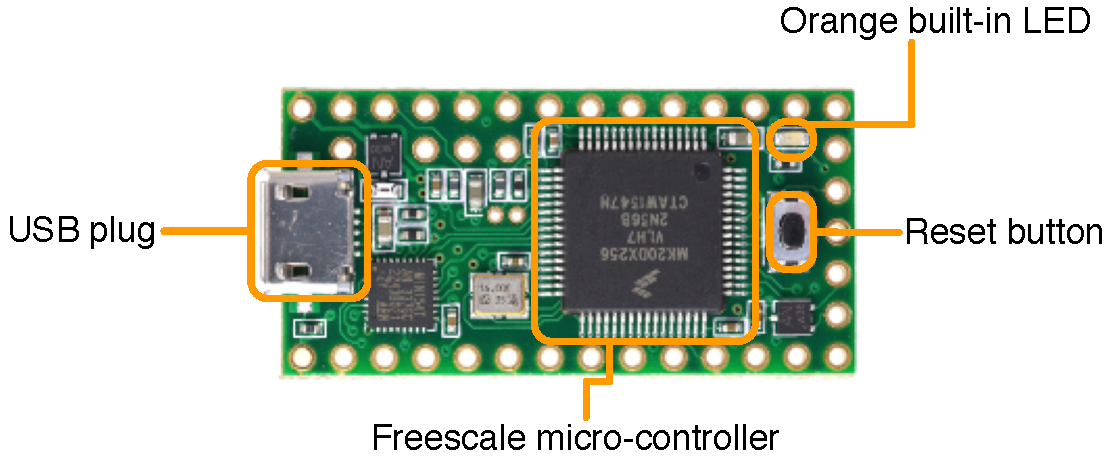
\includegraphics[scale=0.5]{teensy31.pdf}
\end{center}

\section{The labs board}

The labs board put together the following systems:
\begin{itemize}
\item A 20 colums, 4 lines LCD screen;
\item 5 push buttons;
\item 5 red LEDs;
\item A Quadrature encoder with a push button;
\item A PWM\footnote{Pulse Width Modulation} output / analog input;
\item A green LED to display the PWM.
\end{itemize}

Here is a picture of the board:

\begin{center}
\noindent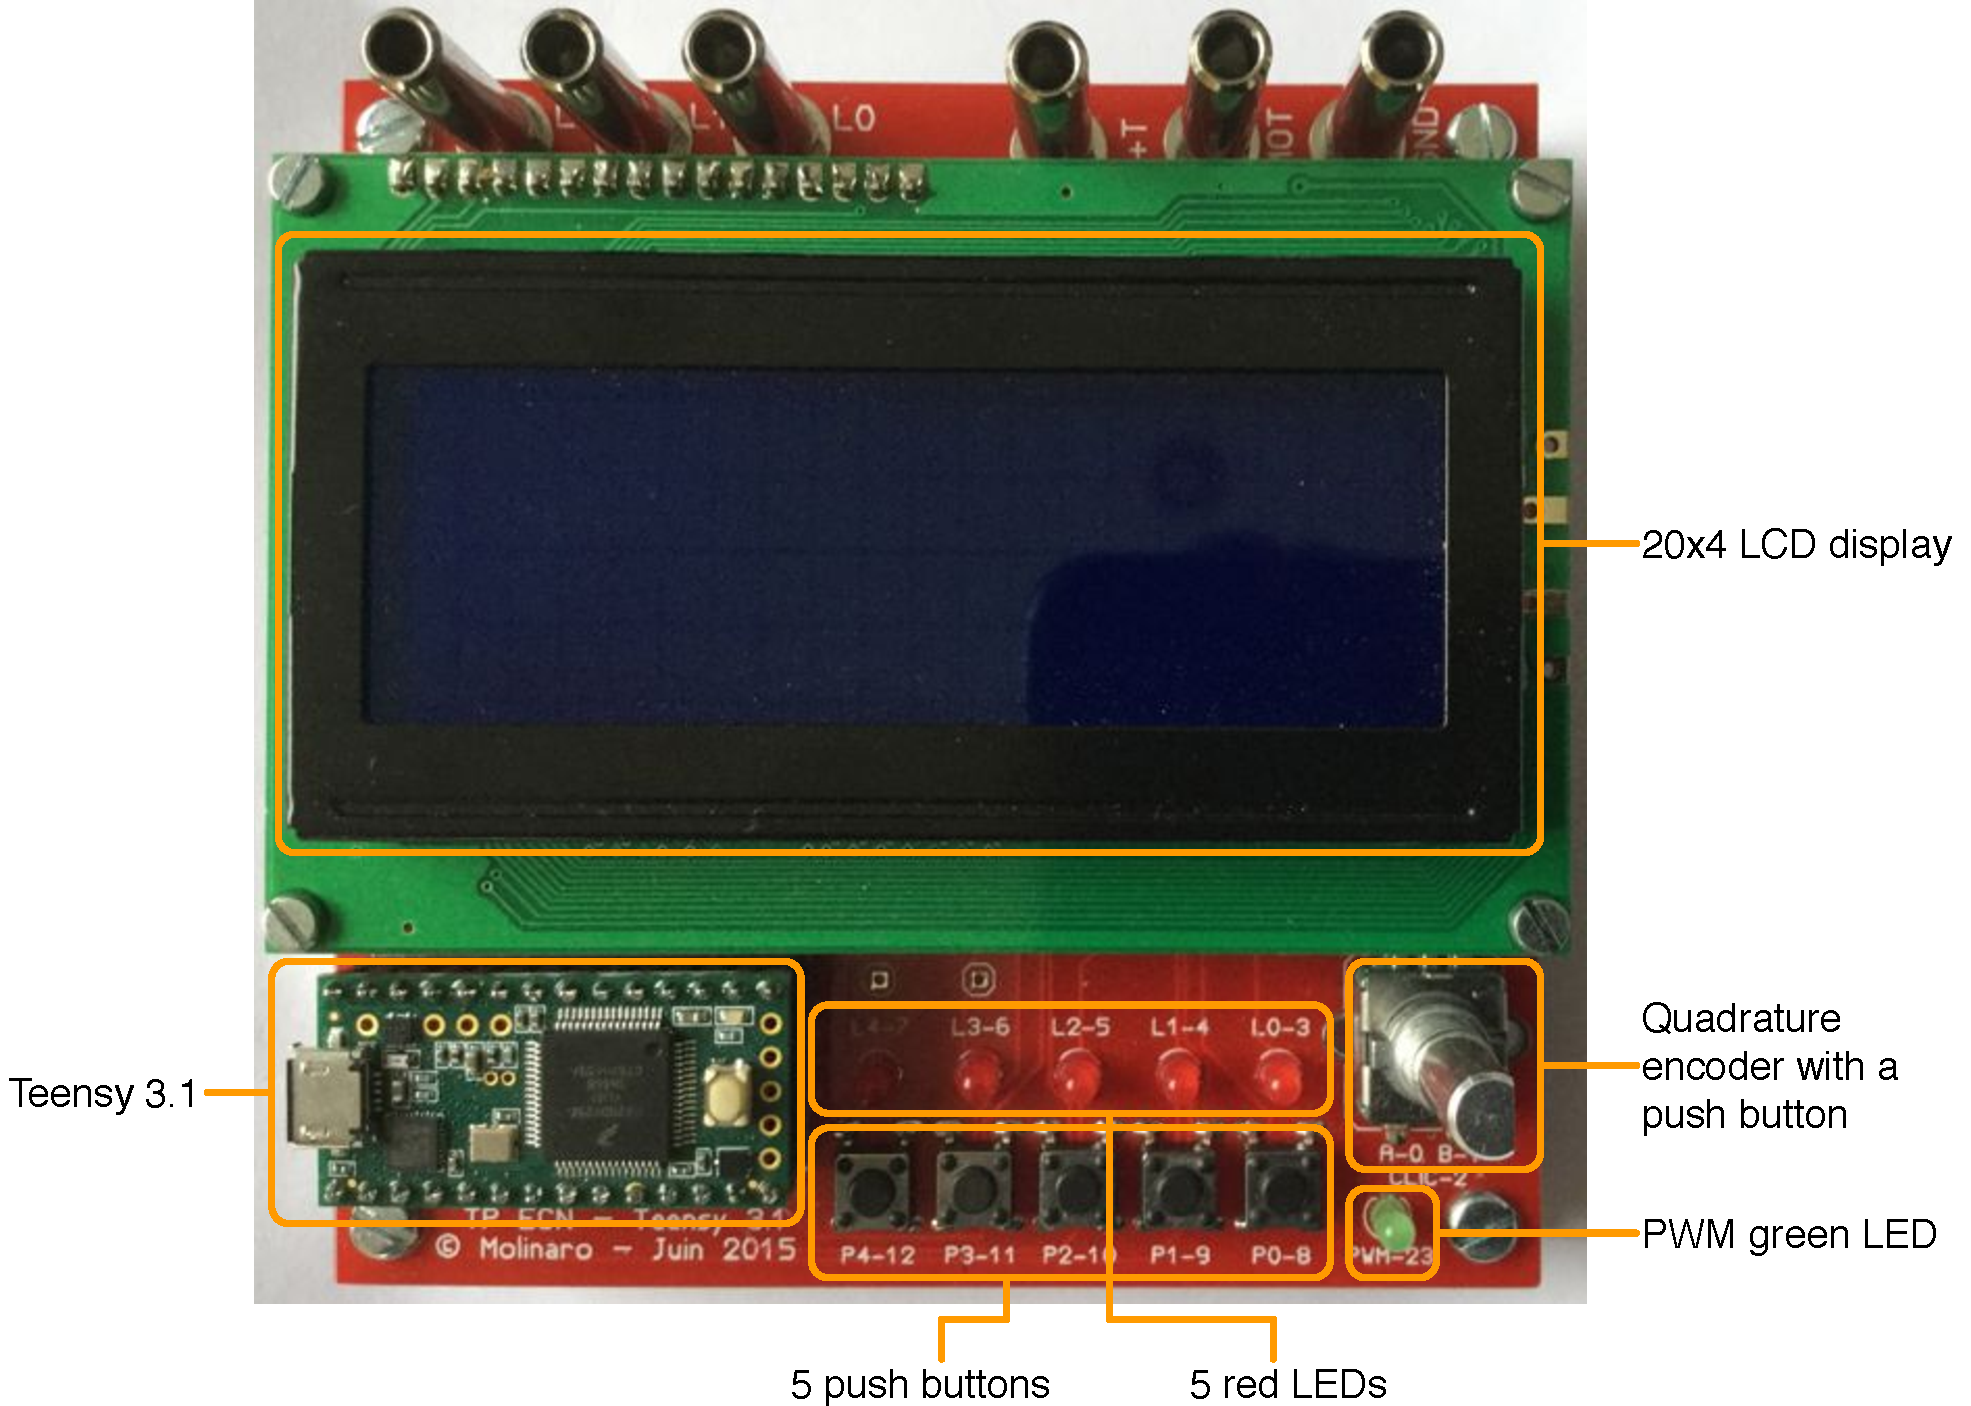
\includegraphics[scale=0.45]{labsboard.pdf}
\end{center}

The board power is supplied by the USB. Connect a USB  port to the Teensy USB plug and the board switches on.

\section{LEDs, buttons and LCD}

The Trampoline port for this board includes functions to turn LED on and off, to read the buttons and to write to the LCD. These functions work as the functions available on an Arduino:

\begin{description}

\item[void pinMode({\it pin}, {\it mode})] sets the mode of a pin. {\it pin} is the number of the pin and {\it mode} can be {\tt INPUT}, the pin is an input, {\tt INPUT_PULLUP}, the pin is an input and a resistor pulls the pin up to 3.3V (logical 1), {\tt OUTPUT}, the pin is an output.

\item[uint8 digitalRead({\it pin})] returns the logical level of a pin: HIGH (logical 1) or LOW (logical 0). {\it pin} is the number of the pin. If the pin is programmed as an input, the value is what is set on the external pin. If the pin is programmed as an output, the value is what was written to the pin.

\item[void digitalWrite({\it pin}, {\it state})] set the logical level of a pin \emph{or} enable or disable the pullup. {\it pin} is the number of the pin, {\tt state} is the logical level:  {\tt HIGH} (logical 1) or {\tt LOW} (logical 0). If the pin is programmed as an output, the state is set on the external pin. If the pin is programmed as an input, a {\tt HIGH} state enables the pullup, a {\tt LOW} state disables the pullup.

\end{description}

The LCD is accessed by using the LiquidCrystalFast library which is compatible with the LiquidCrystal library. \href{https://www.arduino.cc/en/Reference/LiquidCrystal}{You can get the documentation here}.

\subsection{LEDs}

If you look just above the LEDs, you see labels {\tt Lx-y}. {\tt L} means {\bf L}ED, {\tt x} is the identifier of the LED and {\tt y} is the number of the Teensy pin  used to control the state of the LED.

\begin{center}
\noindent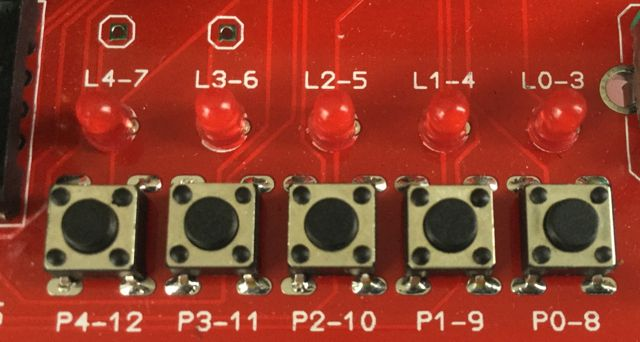
\includegraphics[scale=0.35]{ledsbuttons.jpg}
\end{center}

To use a LED, you need to:
\begin{enumerate}
\item Program the corresponding pin, {\tt y}, as an output;
\item Set the logical level to {\tt HIGH} to turn the LED on;
\item Set the logical level to {\tt LOW} to turn the LED off;
\end{enumerate}

Typically, pin direction programming is done in the {\tt main} function before starting Trampoline. For instance the following source code turns on LED 0 (pinMode and digitalWrite on pin 3) before to start Trampoline by calling the StartOS function.

\begin{lstlisting}[language=C]
int main()
{
    pinMode(3, OUTPUT);    /* LED L0-3 pin is set as an output */
    digitalWrite(3, HIGH); /* Turn L0-3 on                     */

    /* Start Trampoline in the default appmode */
    StartOS(OSDEFAULTAPPMODE);
    return 0;
}
\end{lstlisting}

\subsection{Pushbuttons}

As for LEDs, pushbuttons are labelled with {\tt Px_y} where {\tt P} stands for {\bf P}ushbutton, {\tt x} is its number and {\tt y} is the number of the Teensy pin used to read the state of the pushbutton.

When pushed, a pushbutton connects the corresponding pin to the ground producing a logic 0 state (LOW). When not pushed, the pin is floating. i.e. it is not connected to anything.

Tu use a pushbutton, you need to:
\begin{enumerate}
\item Program the corresponding pin, {\tt y}, as an input with pullup enabled;
\item Read the pin, {\tt y}, to be informed of the state of the pushbutton:
    \begin{itemize}
        \item if the returned value is {\tt HIGH} the button is not pushed;
        \item if the returned value is {\tt LOW} the button is pushed;
    \end{itemize}
\end{enumerate}

The following example reads button {\tt P0_8} to start Trampoline in a specific appmode.

\begin{lstlisting}[language=C]
int main()
{
    pinMode(8, INPUT_PULLUP);  /* Button P0_8 pin is set as
                                  an input with pullup enabled */
    if (digitalRead(8) == LOW) /* The button is pressed        */
    {
      /* Start Trampoline in the testAppmode appmode */
      StartOS(testAppmode);
    }
    else                       /* otherwise */
    {
      /* Start Trampoline in the default appmode */
      StartOS(OSDEFAULTAPPMODE);
    }
    return 0;
}
\end{lstlisting}

\subsection{LCD}

As already stated, the LCD is driven by the LiquidCrystalFast library. This library is written in C++. An object of type LiquidCrystalFast is instantiated with the connection pins as arguments. The LCD is connected to pins 18,17,16,15,14 and 19. So a LiquidCrystalFast object must be instantiated as a global variable as follow:

\begin{lstlisting}[language=C]
/*
 * A LiquidCrystalFast object is instantiated.
 * Pin numbers are per Teensyduino specification
 */
LiquidCrystalFast lcd(18,17,16,15,14,19);
\end{lstlisting}

In the main function, the LCD is initialized by using the following instruction:

\begin{lstlisting}[language=C]
  lcd.begin(20, 4);
\end{lstlisting}

20 is the number of columns and 4 the number of lines. Once the LCD has been initialized, the following methods can be used:
\begin{description}
\item[lcd.setCursor({\it x}, {\it y})] to put the cursor at column {\it x} and line {\it y};
\item[lcd.print({\it something})] to write {\it something} on the LCD;
\item[lcd.println({\it something})] to write {\it something} on the LCD and go at the beginning of the next line.
\end{description}

\chapter{Lab 1 -- Understanding fixed priority scheduling}

\section{Goal}

The goal of this lab is to become familiar with OSEK/VDX applications development process and with Trampoline and to understand how fixed priority scheduling works.
We will also see Hook Routines and Events.
Trampoline is a Free Software implementation of the OSEK/VDX specification.
Trampoline includes an OIL compiler which allows, starting from an OIL description, to generate OS level data structures of the application.
In addition to the OIL description, the developer must provide the C sources of tasks and ISRs implementing the application.

Get the lab1 starting source files. Go at \url{http://www.irccyn.ec-nantes.fr/~bechenne/trampoline-labs/} and get the first archive. Once downloaded it expands to a lab1 directory.

\section{Starting point}

Go into the lab1 directory. There are 2 files:

\begin{description}
\item[lab1.oil] the OIL description of the lab1 application.
\item[lab1.cpp] the C++ source for the lab1 task and hook routines (C++ is needed because of LiquidCrystalFast library).
\end{description}

Edit the lab1.oil and look at the \texttt{TRAMPOLINE_BASE_PATH} attribute (in OS $>$ BUILD attribute).
It should point to the directory where Trampoline is installed.
Set it to: \texttt{/usr/local/tp_treel_imta/trampoline}.

You should also modify the \texttt{LDFLAGS} lines describing the location of the libraries used by the cross compiler. Set the first line to:

{\footnotesize
\begin{verbatim}
-L/usr/local/tp_treel_imta/gcc-arm-none-eabi-7-2018-q2-update/arm-none-eabi/lib/thumb/v7e-m
\end{verbatim}}

and the second one to:

{\footnotesize
\begin{verbatim}
-L/usr/local/tp_treel_imta/gcc-arm-none-eabi-7-2018-q2-update/lib/gcc/arm-none-eabi/7.3.1/thumb/v7e-m
\end{verbatim}}


lab1 is a very simple application with only 1 task called {\tt a_task}. {\tt a_task} starts automatically (\texttt{AUTOSTART = TRUE \{ ... \}} in the OIL file). Look at the OIL file and the C source file.

To compile this application, go into the lab1 directory and type:

%\unixcl{\parbox{230\unitlength}{export\blanc{}PATH=\$PATH\textbackslash\\
%:\normaltilde/trampoline/goil/makefile-macosx\textbackslash\\
%:\normaltilde/Tools/gcc-arm/gcc-arm-none-eabi/bin\textbackslash\\
%:\normaltilde/Tools/bin}}

\unixcl{\parbox{\linewidth}{%
goil\blanc{}--target=cortex/armv7/mk20dx256/teensy31\textbackslash\\
--templates=/usr/local/tp_treel_imta/trampoline/goil/templates\blanc{}lab1.oil}}

The \texttt{--target} option gives the target system (here we generate the OS level data structures of Trampoline for a {\tt cortex} core with the {\tt armv7} instruction set, a {\tt mk20dx256} micro-controller and the board is a {\tt teensy}).
The \texttt{--templates} option indicates to Goil where to find the template files used to generate the C code of the configuration of the kernel.
The OIL file gives the names of the C source files (with \texttt{APP_SRC} for a C file or \texttt{APP_CPPSRC} for a C++ file) and the name of the executable file (with \texttt{APP_NAME}).

Alongside the C files of the kernel configuration, Goil generates a build script for the application (files {\tt make.py} and {\tt build.py}).

If you change something in the OIL file or in your C++ file, you should not need to re-run Goil because the build script will run it when needed.

Continue the build process by typing:

\unixcl{./build.py}

The application and Trampoline OS are compiled and linked together.
The target file is named \texttt{lab1_exe}.

To upload the application to the Teensy, check that the board is connected to the computer, then type:

\unixcl{./build.py\blanc{}burn}

The following message is displayed:

\begin{shaded*}
\scriptsize
\vspace{-1.7mm}
\begin{verbatim}
Teensy Loader, Command Line, Version 2.0
Read "lab1_exe.hex": 12660 bytes, 4.8% usage
Waiting for Teensy device...
 (hint: press the reset button)
\end{verbatim}
\end{shaded*}

Press the reset button of the Teensy. Teensy loader uploads the binary to the flash of the micro-controller and displays:

\begin{shaded*}
\scriptsize
\vspace{-1.7mm}
\begin{verbatim}
Found HalfKay Bootloader
Read "lab1_exe.hex": 12660 bytes, 4.8% usage
Programming.............
Booting
\end{verbatim}
\end{shaded*}


The program starts and the following message should be displayed on the LCD (the first line corresponds to the execution of the main and the second line corresponds to the execution of task a_task). In addition, task a_task turns on all the LEDs.

\begin{center}
   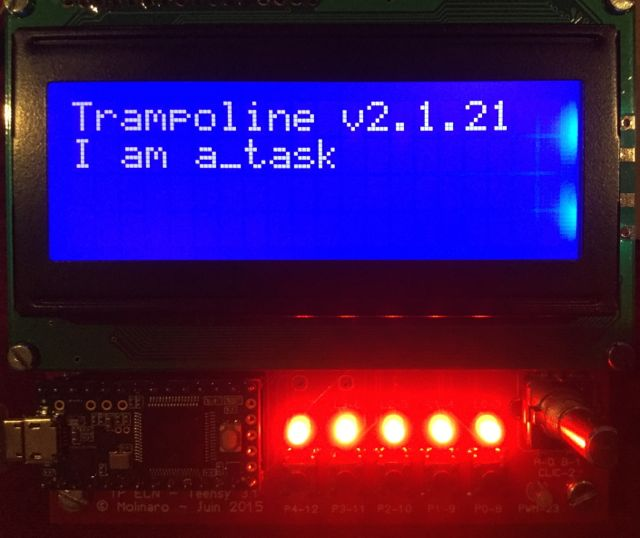
\includegraphics[scale=0.5]{iamatask.jpg}
\end{center}

\subsection{A word about memory sections}

AUTOSAR defines a way to put objects (constants, variables and functions) in memory sections in a portable way\footnote{memory section declaration is not part of the C standard}. For that, a set of macro are used along with a generated file: MemMap.h. Functions should be declared with the \lstinline{FUNC} macro, variables with the \lstinline{VAR} macro, constants with the \lstinline{CONST} macro and pointers to variables, pointers to constant, constant pointers to variable and constant pointers to constant with \lstinline{P2VAR}, \lstinline{P2CONST}, \lstinline{CONSTP2VAR} and \lstinline{CONSTP2CONST} respectively. Sections are opened and closed with a macro definition and the inclusion of the \lstinline{tpl_memmap.h} file. For instance:

\begin{lstlisting}
#define APP_Task_my_periodic_task_START_SEC_VAR_32BIT
#include "tpl_memmap.h"
VAR(int, AUTOMATIC) period;
VAR(int, AUTOMATIC) occurence;
#define APP_Task_my_periodic_task_STOP_SEC_VAR_32BIT
#include "tpl_memmap.h"
\end{lstlisting}

defines variables \lstinline{period} and \lstinline{occurence} in the variables section of task \lstinline{my_periodic_task}.

\begin{lstlisting}
#define APP_Task_my_periodic_task_START_SEC_CODE
#include "tpl_memmap.h"
TASK(my_periodic_task)
{
  ...
  TerminateTask();
}
#define APP_Task_my_periodic_task_STOP_SEC_CODE
#include "tpl_memmap.h"
\end{lstlisting}

defines the task \lstinline{my_periodic_task} in the code section of task \lstinline{my_periodic_task}. \lstinline{goil} generates the sections for tasks according to the description.


\section{OS system calls and tasks}

\subsection{Task activation and scheduling}

The \texttt{ActivateTask()} system call allows to activate a task of the application.

\begin{ex}
    Add two tasks in the system: \texttt{task_0} and \texttt{task_1}.
    \begin{itemize}
        \item add the declaration of both tasks in the OIL file; \texttt{task_0} should have priority 1 and its AUTOSTART attribute should be set to FALSE; \texttt{task_1} should have priority 8 and its AUTOSTART attribute should be set to FALSE;
        \item in the cpp file, you should:
            \begin{itemize}
                \item declare both tasks with the DeclareTask keyword,
                \item provide the body of both tasks: each task prints its name on a line of the LCD and then terminates,
                \item and, lastly, modify the body of task \texttt{a\_task} to activate \texttt{task_0} and \texttt{task\_1} (in this order).
            \end{itemize}
    \end{itemize}

    Before to execute the resulting application, draw a schedule.
    Your diagram must clearly show activation, execution and termination of each job.
    Then execute the application and check the correctness of your diagram.
\end{ex}

\subsection{Task chaining}

The \texttt{ChainTask()} system call allows to chain the execution of a task: the calling job terminates and a new job of the target task is created.

\begin{ex}
Replace the call to \texttt{TerminateTask} by a \texttt{ChainTask(task_1)} at the end of task a task.
Draw a schedule of the new system.
Then execute the application to check the correctness of your diagram.
Comment on the differences with the previous application.
\end{ex}

\begin{ex}
Chain to \texttt{task_0} instead of \texttt{task_1}.
Draw a schedule of the new system.
Then execute the application to check the correctness of your diagram.
Comment on the differences with the previous application.
\end{ex}

\begin{ex}
Test the error code returned by ChainTask.
Modify the OIL file so that ChainTask returns \texttt{E\_OK}.
Draw a schedule of the new system.
Then execute the application to check the correctness of your diagram.
Comment on the differences with the previous application.
\end{ex}

\section{Extended tasks and synchronization using events}

Unlike a basic task, an extended task may wait for an event.
In terms of scheduling, a job is activated when a task is activated or when it leaves the waiting state.

Before to proceed with the following questions, consult the slides of the course to become familiar with events in Trampoline.

%In the OIL file, set the priority of \texttt{task_0} to 8 and add two events \texttt{evt_0} and \texttt{evt_1}. \texttt{evt_0} is used by \texttt{task_0} and \texttt{evt_1} is used by \texttt{task_1}. \texttt{a_task} activates \texttt{task_0} and \texttt{task_1} then sets \texttt{evt_0} and \texttt{evt_1} and terminates. \texttt{task_0} and \texttt{task_1} wait for their event, clear it and terminate.

\begin{ex}
     Modify the application of Question~1:
\begin{itemize}
    \item set priority of \texttt{task_0} to 8;
    \item add two events, \texttt{evt\_0} and \texttt{evt\_1}:
        \begin{itemize}
            \item \texttt{evt_0} is set by task \texttt{a\_task} to task \texttt{task\_0}
            \item \texttt{evt_1} is set by task \texttt{a\_task} to task \texttt{task\_1}
        \end{itemize}
    \item modify the body of the tasks:
        \begin{itemize}
            \item task \texttt{a\_task} activates \texttt{task\_0} and \texttt{task\_1} then sets \texttt{evt\_0} and \texttt{evt\_1} before to terminates.
            \item task \texttt{task\_0} and \texttt{task\_1} wait for their event, clear it, and terminate.
        \end{itemize}
\end{itemize}

Draw a schedule of the new system.
Then execute the application to check the correctness of your diagram (before to run the application, add outputs in the bodies of the task, for instance writes to the LCD or LEDs to ease the correctness checking).
Comment on the differences with the previous application.

\end{ex}

\begin{ex}
Program an application conforming to the following requirements:

\begin{itemize}
    \item it is composed of two tasks: \texttt{server} priority 2, \texttt{t1} priority 1.
    \item \texttt{server} is an infinite loop that activates \texttt{t1} and waits for event \texttt{evt_1}.
    \item \texttt{t1} prints ``I am t1'' and sets \texttt{evt_1} of \texttt{server}.
\end{itemize}

Before to run the application, draw a schedule of the execution. Add outputs in the bodies of the task (for instance writes to the LCD or the LEDs) to verify your schedule.
\end{ex}

\begin{ex}
Extend the previous application by adding 2 tasks: \texttt{t2} and \texttt{t3} (priority 1 for both) and 2 events \texttt{evt_2} and \texttt{evt_3}. \texttt{server} activates \texttt{t1}, \texttt{t2} and \texttt{t3} and waits for one of the events. When one of the events is set, \texttt{server} activates the corresponding task again.


Before to run the application, draw a schedule of the execution. Add outputs in the bodies of the task (for instance writes to the LCD or the LEDs) to verify your schedule.
\end{ex}

%================================================================
\chapter{Lab 2 -- Periodic tasks and Alarms}

\section{Goal}

Real-Time systems are reactive systems which have to do processing as a result of events. You have seen in Lab \#1 how to start processing as a result of an internal event of the system: by activating a task (\texttt{ActivateTask} and \texttt{ChainTask} services) or by setting an event (\texttt{SetEvent} service). In this lab, you will trigger processing as a result of time elapsing (expiration of an Alarm). This lab uses the following concepts: alarm and counter. On the lab board, the Systick timer is used as interrupt source for alarms. The interrupt is sent every 1ms.

Go to \url{http://www.irccyn.ec-nantes.fr/~bechenne/trampoline-labs} and download the lab2 package.

\section{First application}

This application implements a periodic task that reads push button P0_8 of the board every 100ms.
When button P0_8 is pushed, led L0_3 is turned on.
When button P0_8 is released, led L0_3 is turned off.

\begin{ex}
The {\tt readButton} function implements a small state machine to convert the state of the button to states and events.
Draw this state machine.
Draw a schedule of the application (the execution of the interrupt service routine associated with the timer will not be represented; it will be assumed to be negligible).
Your diagram should show pressing and releasing events of button P0_8 as well as the state of led L0_3.
Build and execute the application to verify your diagram.
\end{ex}

Modify the application: when P0_8 is pushed, a processing is triggered.
This processing is performed by activating a job of task \texttt{t_process} (priority 3) that, on odd executions, displays the message \textsl{``processing triggered"}, and, on even executions, clears the LCD.
\begin{ex}
Draw a schedule of the application.
Your diagram should show pressing and releasing events of of button P0_8 as well as the state of the LCD (associate numbers with the different state and use these numbers in your diagram).
Build and execute the application to verify your diagram.
\end{ex}


\section{Second application}

The second application will use 2 periodic tasks: \texttt{t1} (priority 2, period 1s) and \texttt{t2} (priority 1, period 1.5s). t1 toggles LED L0_3 each time it executes and t2 toggles LED L1_4.

\begin{ex}
    Draw a schedule of the application that show the 20 first states of the LED.
    What is the global period of the system?
\end{ex}

The application needs a counter and 2 alarms. Program, build, and run the application.

\begin{ex}
What is the maximal value that can be used for the \texttt{TICKSPERBASE} variale to fulfill the application requirements?
How are the alarms configured to fulfill the application requirements?
\end{ex}

\section{Third application}

In the third application, alarms, counters, and polling of the push buttons are mixed.
This application is a system with 2 push buttons.
After starting the system waits.
When the first button is pressed, the system starts a {\it function}\footnote{Here we mean a function of the application, not a function of the C language.} F that is implemented using a periodic task (period = 1s).
To ``see'' F, uses a blinking LED as in the second application.
When the first button is pressed again, function F is stopped.
When the second button is pressed, the system is shutdown as quickly as possible (ie ShutdownOS\footnote{The ShutdownOS service shutdowns the operationg system. All tasks and alarms are stopped. ShutdownOS takes a StatusType argument to specify the kind or error which occurred. In our case use E_OK as argument.} is called).

\begin{ex}
    Explain the design of the application: provide the list and configuration of tasks and alarms.
    Draw schedules showing different execution scenarii.
    Build and execute the application to verify your diagrams.
\end{ex}

Requirements change. Now function F implementation needs an Init code
(runs once when the F is started) and a Final code (runs once when F is stopped) as shown in the following diagram:

\begin{center}
\begin{adjustbox}{width=14cm,keepaspectratio}
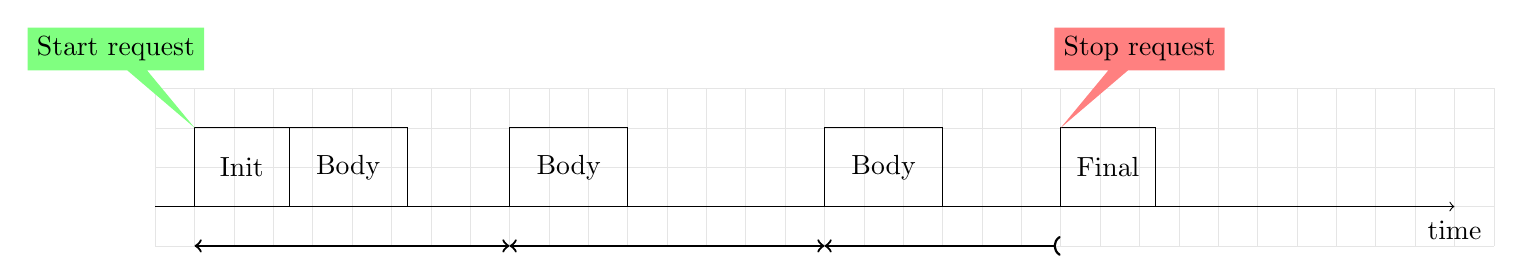
\begin{tikzpicture}
\draw[step=.5cm,gray!20,very thin] (-0.5, -0.5) grid (16.5,1.5);
\draw [->] (-0.5,0) -- (16,0);
\node [yshift=-3mm] at (16,0) {time};
\draw (0,0) rectangle (1.2,1);
\node at (0.6,0.5) {Init};
\draw (1.2,0) rectangle (2.7,1);
\node at (1.95,0.5) {Body};
\draw (4,0) rectangle (5.5,1);
\node at (4.75,0.5) {Body};
\draw (8,0) rectangle (9.5,1);
\node at (8.75,0.5) {Body};
\foreach \x in {0, 4}
  \draw [xshift=\x cm,thick,<->] (0,-0.5) -- (4,-0.5);
\draw [xshift=8 cm,thick,<-(] (0,-0.5) -- (3,-0.5);
\draw [xshift=11cm] (0,0) rectangle (1.2,1);
\node [xshift=11cm] at (0.6,0.5) {Final};
\node [rectangle callout, fill=green!50, callout absolute pointer={(0,1)}] at (-1,2) {Start request};
\node [rectangle callout, fill=red!50, callout absolute pointer={(11,1)}] at (12,2) {Stop request};
\end{tikzpicture}
\end{adjustbox}
\end{center}


\begin{ex}
    Modify the application to take the new requirements into account.
    Your implementation will use only basic tasks.
    Explain the design of the application: provide the list and configuration of tasks and alarms.
    Draw schedules showing different execution scenarii.
    Build and execute the application to verify your diagrams.
\end{ex}

\begin{ex}
    Same question as above, but your implementation will use an extended task to control the execution of Init, F, and Stop.
\end{ex}

\section{Fourth application}

In this part, you will implement a watchdog. It is a mechanism that allows to stop a processing or a waiting period once a delay has elapsed.

In your application, each time P0_8 is pressed, P1_9 must be pressed within 2 seconds. In this case, you print the time between the two occurrences. Otherwise, an error message is displayed. If 2 or more P0_8 are got within 3 seconds from the first one they are ignored.

\begin{ex}
    Specify this behaviour with a state machine.
    What is happening if the timeout occurs just after P1_9 has been pressed but before the waiting task got the event?
    Design and program a solution that handles this situation correctly.
    Draw a schedule of the behaviour of your application in such a scenario (this schedule should show the state of the alarms).
\end{ex}

\section{Fifth application}

Program a chase\footnote{chenillard in French} with a 0.5s period. To do so, use 4 periodic tasks. Each periodic task manages a LED. The chase effect is done by using alarms with a time shift between them.

When P0_8 is pressed, the chase stops.
When P1_9 is pressed, the chase resumes from the states where it was stopped.
When P2_10 is pressed, the chase direction changes (even if it is stopped).

\begin{ex}
    Specify the high level behaviour with a state machine.
    Design and program the application.
    Explain your design.
\end{ex}

%================================================================
\chapter{Lab 3 -- Shared object access protection}

To show resources usage, we will use a bad program that allows to corrupt a shared global variable which is not protected against concurrent writes. This has been presented in the course. This lab will show different ways to prevent this wrong behavior by using resources (standard and internal) or other solutions (preemption and priority).

Get the lab3 package directory from \url{http://www.irccyn.ec-nantes.fr/~bechenne/trampoline-labs}.

\section{Application requirements}

The diagram of figure~\ref{fig:appdiag} describes the application.
It is composed of 3 tasks that share 2 global variables {\bf declared with the volatile keyword}: \texttt{val} and \texttt{activationCount}:
\begin{itemize}
\item a background task called \texttt{bgTask}, with a job activated at system startup (\texttt{AUTOSTART = TRUE}) that never ends. In an infinite loop it increments then decrements the global variable \texttt{val}. This task has priority 1.
\item a periodic task called \texttt{periodicTask} that activates a job every 100ms\footnote{a counter gets a tick every 10ms}. This periodic task increments the global variable \texttt{activationCount}. If \texttt{activationCount} is odd, \texttt{val} is incremented, otherwise it is decremented.
\item a periodic task \texttt{displayTask} that runs every second and prints on the standard output \texttt{val} and \texttt{activationCount}.
\end{itemize}

\def\alarm#1#2{
  \node[alarm](#1) [#2] {};
  \coordinate (a) at ($(#1.north)$);
  \coordinate (b) at ($(#1.north east)$);
  \coordinate (c) at ($(#1.north west)$);
  \coordinate (d) at ($(#1)$);
  \draw[thick] ($(a)+(-0.1,0)$) rectangle ($(a)+(0.1,0.1)$);
  \draw[rotate=-45,thick] ($(b)+(-0.05,0)$) rectangle ($(b)+(0.05,0.1)$);
  \draw[rotate=45,thick] ($(c)+(-0.05,0)$) rectangle ($(c)+(0.05,0.1)$);
  \draw ($(d)+(0.3,0)$) -- (d) -- ($(d)+(0,0.3)$);
  \node [font=\scriptsize,below=0.5mm of #1] {{\em Alarm}}
}

\def\sharedvar#1#2#3{
  \node (#1) [#2] {#1};
  \coordinate (a) at ($(#1.north #3) + (0,0.2)$);
  \coordinate (b) at ($(#1.south #3) + (0,-0.2)$);
  \draw[ultra thick] (a) -- (b);
  \draw ($(a)+(-0.1,0)$) -- ($(a)+(0.1,0)$);
  \draw ($(b)+(-0.1,0)$) -- ($(b)+(0.1,0)$)
}

\def\varrect#1{
  \draw ($(#1.south west)$) rectangle ($(#1.north east)$)
}

\begin{figure}[htbp] %  figure placement: here, top, bottom, or page
   \centering
   \begin{tikzpicture}[
   task/.style={draw,very thick,fill=white,drop shadow={opacity=0.25},text width=2.5cm, text centered, minimum height=1.5cm},
   alarm/.style={draw,thick,circle,fill=white,drop shadow={opacity=0.25},text width=.5cm}
   ]
   \node[task](periodicTask) at (0,0) {periodicTask};
   \node[task](bgTask) [above=of periodicTask] {bgTask};
   \node[task](displayTask) [above=of bgTask] {displayTask};
   \alarm{activateDisplay}{left=20mm of displayTask};
   \alarm{activatePeriodic}{left=20mm of periodicTask};
   \sharedvar{val}{left=of bgTask}{east};
   \sharedvar{activationCount}{right=of periodicTask}{west};
   \sharedvar{stdout}{right=of displayTask}{west};
   \varrect{stdout};
   \draw [thick,<->] (val.east) -- (bgTask.west);
   \draw [thick,->] (val.north east) -- ++(5mm,0) |- ($(displayTask.south west) + (0,2mm)$);
   \draw [thick,<->] (val.south east) -- ++(5mm,0) |- ($(periodicTask.north west) + (0,-2mm)$);

   \draw [thick,->] (activateDisplay.east) -- ++(5mm,0) -- ++(0,1.5mm) -- ++(3mm,-3mm) -- ++ (0mm,1.5mm) -- (displayTask);
   \node at ($(activateDisplay.east) + (6.5mm,-3mm)$) {1s};
   \node[font=\scriptsize] at ($(activateDisplay.east) + (9mm,3mm)$) {{\em ActivateTask}};
   \draw [thick,->] (activatePeriodic.east) -- ++(5mm,0) -- ++(0,1.5mm) -- ++(3mm,-3mm) -- ++ (0mm,1.5mm) -- (periodicTask);
   \node at ($(activatePeriodic.east) + (6.5mm,-3mm)$) {100ms};
   \node[font=\scriptsize] at ($(activatePeriodic.east) + (9mm,3mm)$) {{\em ActivateTask}};
   \draw [thick,<->] (activationCount.west) -- (periodicTask);
   \draw [thick,->] (activationCount.north west) -- ++(-5mm,0) |- ($(displayTask.south east) + (0,2mm)$);
   \draw [thick,->] (displayTask) -- (stdout);
   \end{tikzpicture}
   \caption{Application diagram}
   \label{fig:appdiag}
\end{figure}

\begin{ex}
    Before programming the application, gives the expected sequence of values for val.
    Design, program, and run the application.
    Does it conform to the expected one?
    Decrease gradually the period of task \texttt{periodicTask} and observe the sequence of values of val.
    Comment.
\end{ex}


%Compile again your application but add a \unixcl{CFLAGS = "-O3"} in the OIL file. This flag
%makes the C compiler optimize the assembly code.

%\begin{ex}
%Is it the same behavior as in previous question? Why?
%\end{ex}



\section{Global variable protection}

%Remove the \unixcl{CFLAGS = "-O3"} from the OIL file. As shown in the course, we must protect the access to the global variable.

Update the OIL file and the C program to protect the access to the global variable \texttt{val}. Use a resource to do it.

The resource priority is automatically computed by goil according to the priorities of the tasks which use it.

The OIL compiler (goil) generates many files in the directory bearing the same name
as the oil file (without the .oil suffix). Among them 3 are of interest for this lab:
\begin{itemize}
\item \texttt{tpl_app_define.h}
\item \texttt{tpl_app_config.h}
\item \texttt{tpl_app_config.c}
\end{itemize}

The file \texttt{tpl_app_config.c} contains the tasks' descriptors as long as all other data structures. These structures are commented.

\begin{ex} ~
    \begin{itemize}
        \item
            Recall the computation rule of the ceiling priority of a resource with the immediate ceiling protocol.
            According to this rule, what should be the ceiling priority of the resource?
        \item
            Find the actual ceiling priority in \texttt{tpl_app_config.c}. Is it the expected value? If not, is it a problem?
    \end{itemize}
\end{ex}

To observe the impact of the priority ceiling protocol, use the following function to observe the priority of the jobs during their execution. The code is provided in the file \texttt{lab3.c}.

\begin{lstlisting}[language=C]
void displayIdAndCurrentPriority()
{
  TaskType id;
  GetTaskID(&id);
  if (id >= 0)
  {
    tpl_priority prio = (tpl_dyn_proc_table[id]->priority) >> PRIORITY_SHIFT;
    lcd.print("Id=");
    lcd.print(id);
    lcd.print(", Prio=");
    lcd.print(prio);
  }
}
\end{lstlisting}

And you have to add the following line at start of your C file:

\begin{lstlisting}[language=C]
 #include "tpl_os_task_kernel.h"
\end{lstlisting}


\section{Protection with an internal resource}

An internal resource is automatically taken when the job gets the CPU, and released when it terminates. Replace the standard resource by an internal resource in the OIL file. Remove the \texttt{GetResource} and \texttt{ReleaseResource} in the C file.

\begin{ex}~
    \begin{itemize}
        \item
            What happens? Why?
        \item
            How to solve the problem? Draw a schedule of a correct implementation of the system. Program this solution.
    \end{itemize}
\end{ex}


\section{Protection using a single priority level}

\begin{ex}
Modify the OIL file: remove the resource and set the priorities so that no task
can be preempted. Draw a schedule of the system.
\end{ex}

%\chapter{Lab4\\Driving servos}

%The goal of this lab is to build a small application to drive servomotors. Get the lab4 package from \url{http://www.irccyn.ec-nantes.fr/~bechenne/trampoline-labs/}. Inside there are 2 files: \unixcl{servos.h} and \unixcl{servo.cpp}.

%Update Trampoline by going to the trampoline directory and typing \unixcl{git pull}. Compile goil.

%\section{How servos work}

%Servos are driven by using a PWM signal. The width of the signal at the high logic state specifies the position of the servo. The width may range from 0.5ms to 2.5ms for a 180° rotation. In practice servos may not be able to turn by 180° and we are going to use a pulse width ranging from 1ms to 2ms. The signal should repeat every 20ms.

%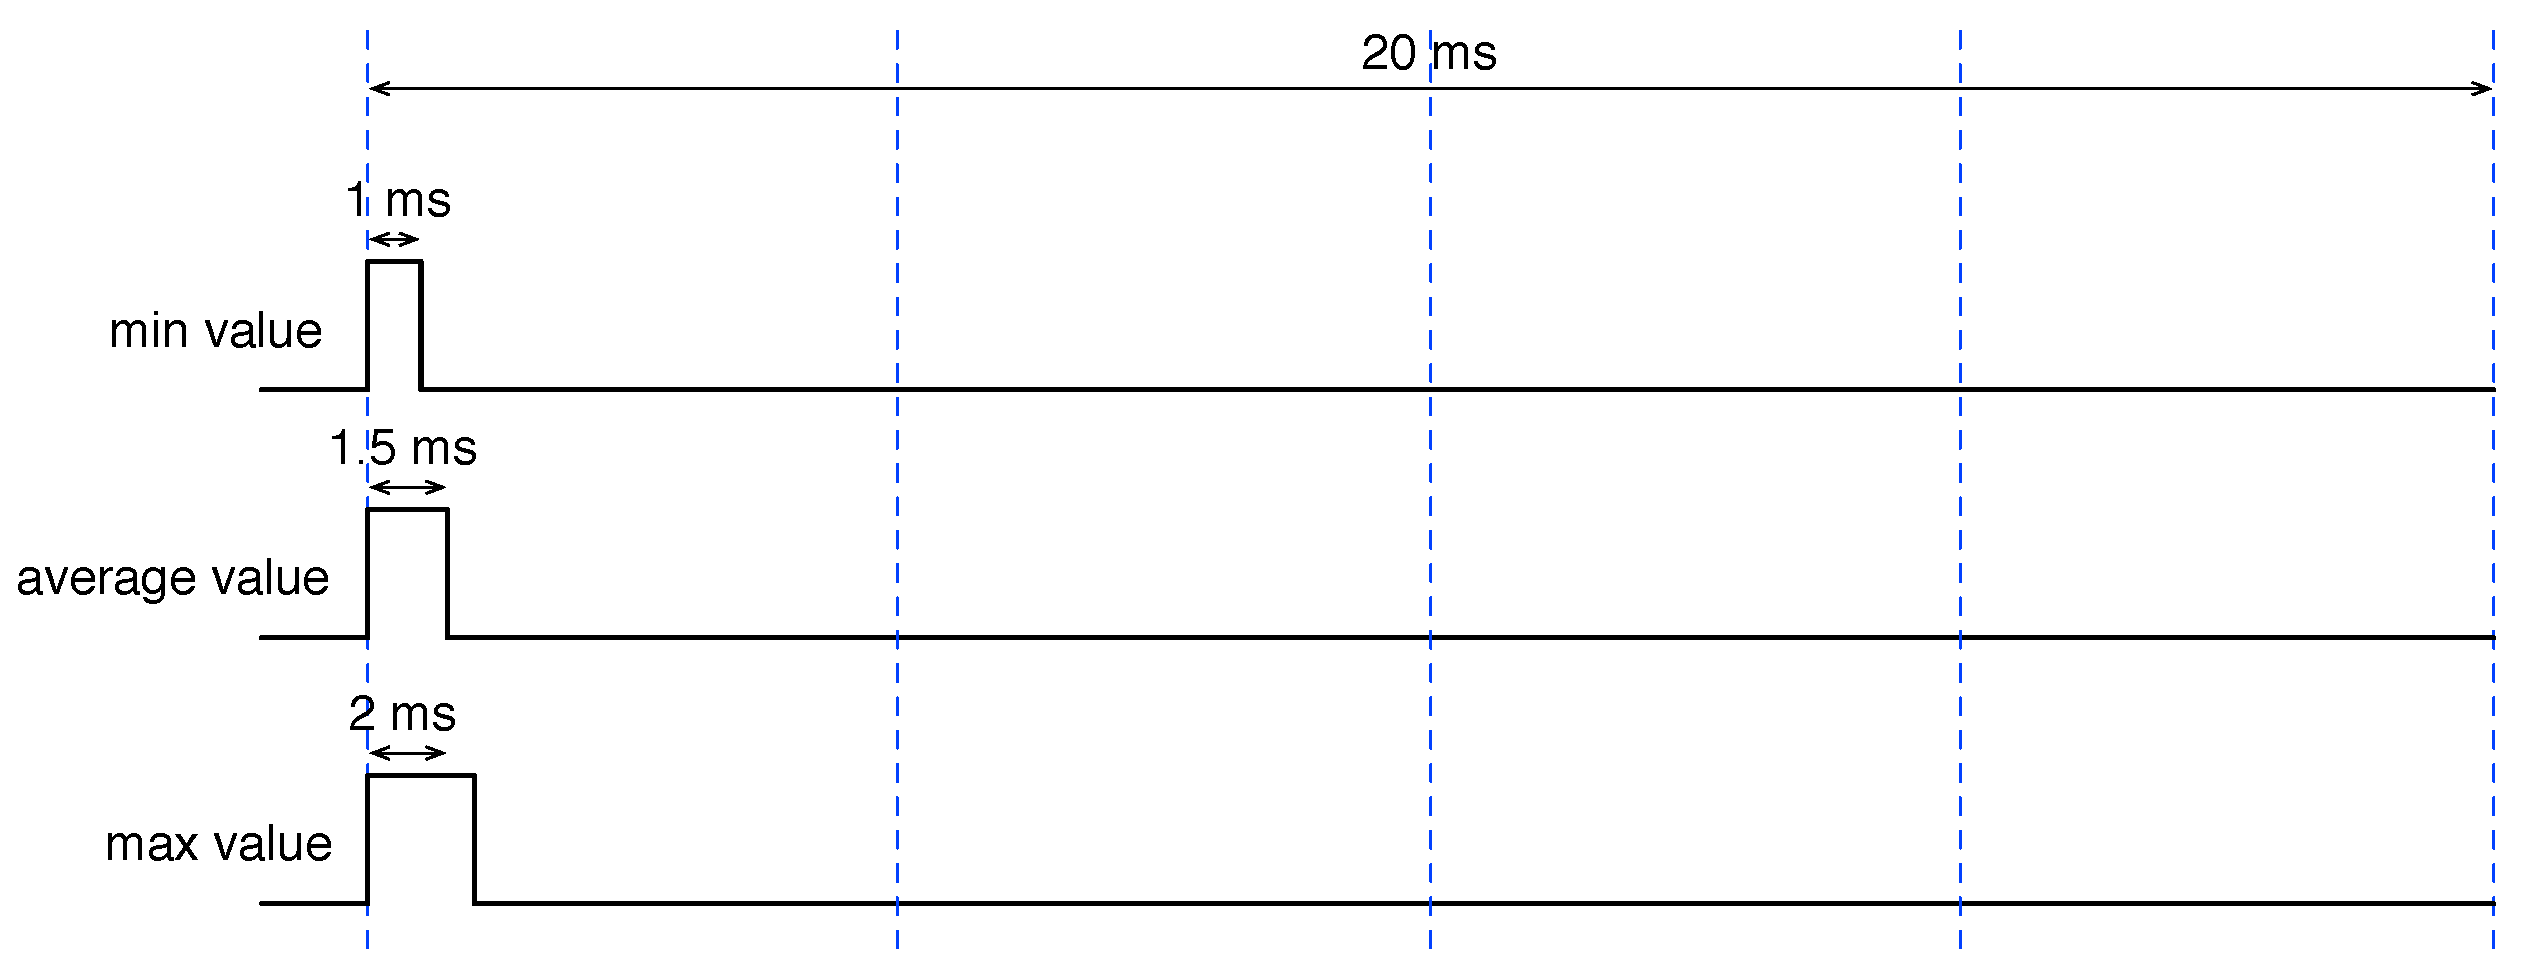
\includegraphics[width=\textwidth]{servopwm.pdf}

%\section{Servo PWM generation}

%The board has 2 connectors for servos on the right side just below the LCD. Servos must be connected with the {\bf yellow wire nearby you} as shown on the picture below.

%\begin{center}
   %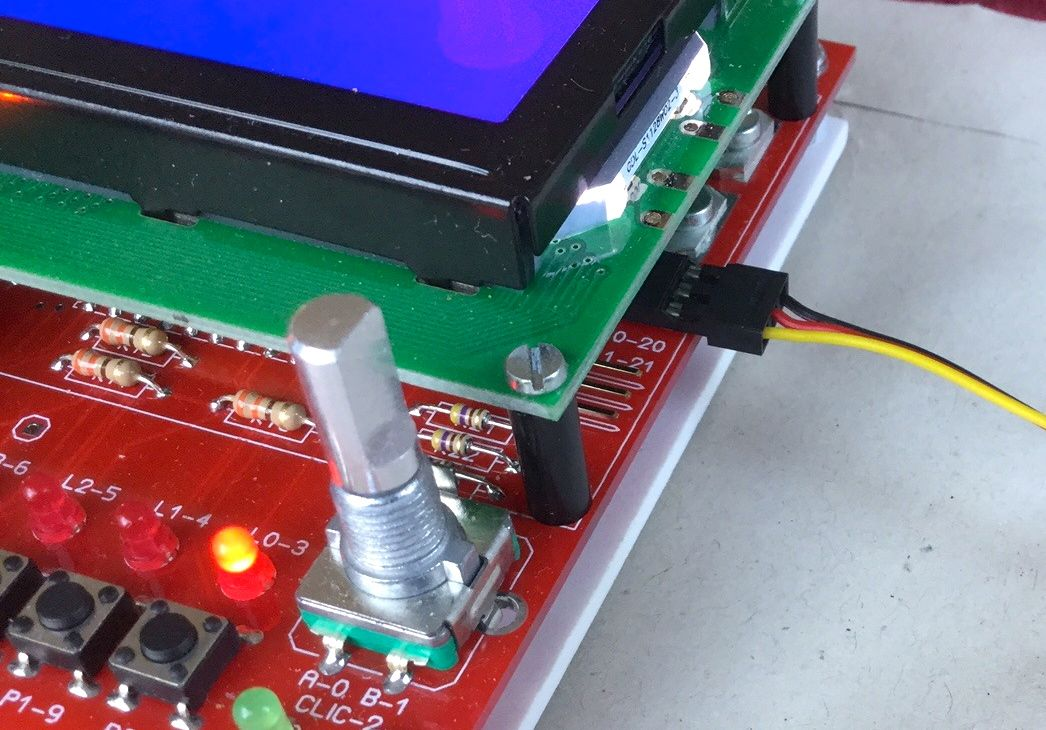
\includegraphics[scale=0.25]{servoconnection.jpg}
%\end{center}

%The 3.3V regulator of the Teensy is not able to power the servos. We need an external power supply connected to the bigs female banana plugs on the top of the board. Get 2 banana cords and connect them to the power supply and to the board as shown on the picture below.

%\begin{center}
   %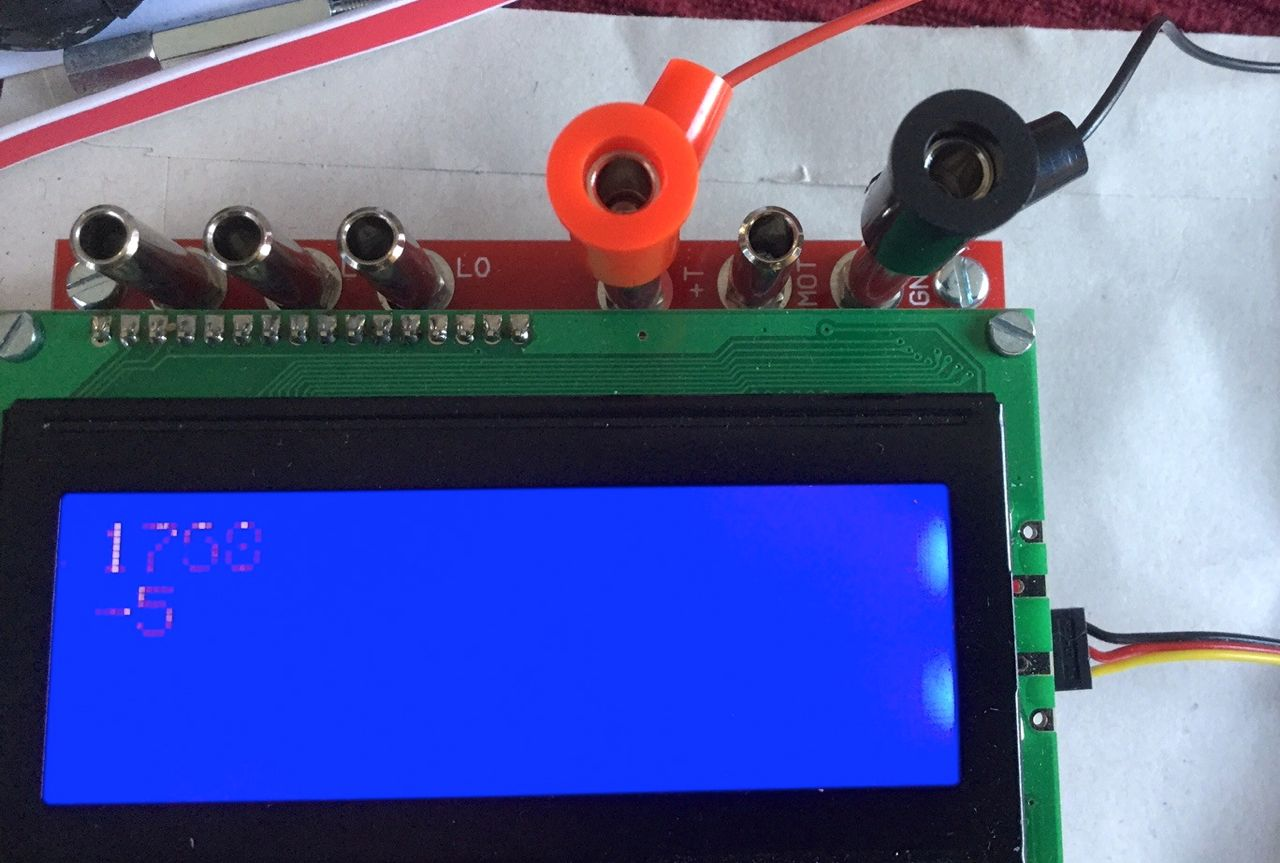
\includegraphics[scale=0.25]{powersupply.jpg}
%\end{center}



%We are going to drive 2 servo. Each servo is driven by a task : \texttt{t_servo0} and \texttt{t_servo1}.

%\begin{ex}
%Program tasks \texttt{t_servo0} and \texttt{t_servo1}. Both tasks are periodic with a 20ms period but are offset by half of the period. \texttt{t_servo0} toggles LED L0-3 and \texttt{t_servo1} toggles LED L1-4. Verify the period using the scope. On the left there is a connector where LED signals are available as well as the GND. Use this connector to connect the scope probes. This connector is shown below
%\end{ex}

%\begin{center}
   %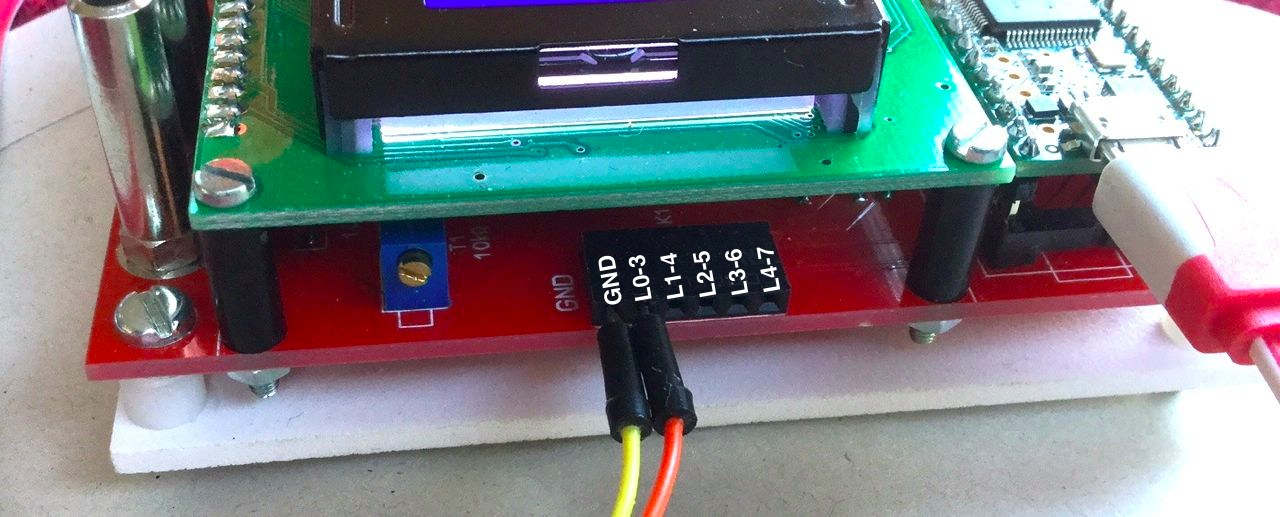
\includegraphics[scale=0.25]{connecteurgauche.jpg}
%\end{center}



%Now instead of toggling the LED, each task will use the function \texttt{pulse}. This function takes 2 arguments. The first one is the \texttt{output}, the second one is the \texttt{duration} of the pulse in $\mu$s.  \texttt{pulse} does not allow values lower than 1000 and greater than 2000 in order to avoid to damage the servo. \texttt{pulse} works as follow: the \texttt{ouput} is set to 1 and a timer of the microcontroller is programmed to generate an interrupt after \texttt{duration} $\mu$s. Since the same timer is used for both tasks, the tasks have to be shifted by at least the maximum duration of the pulse. In your OIL file, you have to declare the ISR which is located in the \texttt{servo.c} file as follow:

%\begin{lstlisting}
  %ISR ftm_timer {
    %CATEGORY = 1;
    %PRIORITY = 1;
    %SOURCE = FTM0_IRQ;
  %};
%\end{lstlisting}

%You have to add the \texttt{servo.c} file in the sources of the application  and the fact you use the ftm library in the BUILD attribute of the OS object:

%\begin{lstlisting}
      %APP_SRC = "servo.c";
      %LIBRARY = ftm;
%\end{lstlisting}

%\begin{ex}
%Modify \texttt{t_servo0} and \texttt{t_servo1} to use \texttt{pulse} and generate a pulse with a width  equal to 1.5ms. Verify the behavior using the scope.
%\end{ex}

%Then change the pins from 3 and 4 to 20 and 21. 20 and 21 correspond to the servo connectors on the right. Connect the servos to the connectors Each servo should go to the average position. Do not forget to program pins 20 an 21 as \texttt{OUTPUT}.

%\section{Adding high level behavior}

%Now we want to set the position of each servo. To do that we need 2 tasks, 1 for each servo, that set the position in a global variable, 1 for each servo. The corresponding variable is read by the \texttt{t_servoX} task to drive the servo.

%\begin{ex}
%First we want the position of each servo incremented until it reaches its maximum position (2ms pulse), then decremented until it reaches its minimum position (1ms pulse). So the servo does round trips. The time we want to go from the minimum position to the maximum position is 5s. Assuming the position is incremented and decremented by one, what is the period of theses tasks in counter tick unit ?
%\end{ex}

%Now we want to be able to set the minimum and maximum positions of the servo connected to pin 20. To do that we use buttons.

%\begin{ex}
%Add to the previous application the following features and draw an automaton to model the application:

%When button P0-8 is pressed, servo connected to pin 20 stops its round-trip. If it is pressed again, round-trip continue. When the round-trip is stopped the following functions are available.

%When button P4-12 is pressed, the minimum position is selected, servo connected to pin 20 goes to this position. Then push buttons P2-10 decrements the minimum position and P1-9 increments the minimum position.

%When button P3-11 is pressed, the maximum position is selected, servo connected to pin 20 goes to this position. Then push buttons P2-10 decrements the minimum position and P1-9 increments the minimum position.

%Minimum position should be kept greater or equal than the position corresponding to the 1ms pulse. Maximum position should be kept lower or equal than the position corresponding to the 2ms pulse. Minimum position should be kept lower or equal than the maximum position.

%When button P0-8 is pressed, servo connected to pin 20 continues its round-trip and respects the minimum and maximum positions that have been set.
%\end{ex}




\end{document}
